\subsubsection{Platformes utilisables pour garantir le fonctionnement de nos algorithmes}
\label{sssec:benchmark}
Malgré que nos algorithmes aient pour but d'être déployés sur l'environnement interne de Thales SE-STAR, il nous a fallu trouver des environnements suffisamment complexes pour tester la robustesse de nos agents mais aussi suffisamment simples pour ne pas devoir attendre un temps infiniment long pour avoir notre réponse. De plus, la connection de nos algorithmes avec SE-STAR est un enjeu essentiel et a apporté son lot de difficulté. Il n'était donc pas raisonnable d'attendre ni de tester nos agents sur cette plateforme.

Il existe de nombreuses plateformes dédiées à l'apprentissage par renforcement. Nous avons choisi de nous concentrer sur des environnements proches de SE-STAR. Ainsi, de nombreuses études en \gls{RL} utilisent des jeux Atari en 2D et 3D. Nous allons donc nous baser en partie sur ce type d'environnement.

Vous pouvez voir page suivante plusieurs types d'environnements sur des plateformes différentes:

\begin{enumerate}
    \item \textbf{Gym\cite{1606.01540} - OpenAI}\\
        Gym est une plateforme qui met à disposition des jeux Atari et des simulations typiques en contrôle (Cartpole, MountainCar ...). La plateforme fournie une \gls{API} permettant de réutiliser nos codes sur l'ensemble des simulations qui sont fournis par Gym.
    
        L'\gls{API} de Gym étant simple, nous avons décider de nous baser sur cette API pour la construction d'un wrapper\footnote{cela consiste en un logiciel intermédiaire qui a pour but de faire le lien entre deux codes.} autour de la simulation interne de Thales SE-STAR.
    
    \item \textbf{Universe - OpenAI}\\
    Universe est une autre plateforme mettant à disposition une multitude de jeux très différents les uns des autres (2D, 3D, textes ...). Certains sont récents et demandent une certaines réflexions (Portal, age of empire, ...). L'organisation de Universe est plus complexe que celle de Gym et impose la prise en compte de plus d'éléments (réseau, possible lag, infrastructure ...). 
    
    Universe propose donc des environnements plus difficiles à tout point de vue que Gym néanmois cette plateforme n'est pas encore utilisé par les chercheurs et on peut douter de la maintenance du projet Universe (OpenAI semble mettre en avant Gym\footnote{Le projet n'a pas été mis à jour depuis 8 mois sur le githubdu projet.})
    
    \item \textbf{DeepmindLab\cite{DBLP:journals/corr/BeattieLTWWKLGV16} - Deepmind / Google }\\
        Le deepmindlab est une seul simulation de labyrinthe 3D très proche de notre application. Le problème est la difficulté d'utilisation de cette plateforme. Ainsi, nous n'avons pas utilisé cette ressource néanmoins elle est pertinante et est une cible pour tester nos algorithmes.
    
    \item \textbf{Doom - Vizdoom\cite{DBLP:journals/corr/KempkaWRTJ16}  }\\
        Doom est un jeu PC de tir à la première personne. Cet environnement est devenu un classique dans la communauté \gls{RL} pour tester les algorithmes d'apprentissage par renforcement. A tel point que l'université de Poznan à créer une compétition d'\gls{IA} basée sur Doom. L'intérêt de cet environnement, contrairement au précédant, est qu'il est plus complet avec un ensemble d'actions possibles conséquent. De plus, l'environnement de Doom met en lumière des difficultés pour les \gls{IA} en matière d'exploration de l'environnement et est donc un terrain de jeu pour résoudre ou proposer des algorithmes résolvant ce type de problème.
    

\end{enumerate}

\bigskip
\begin{figure}
\centering
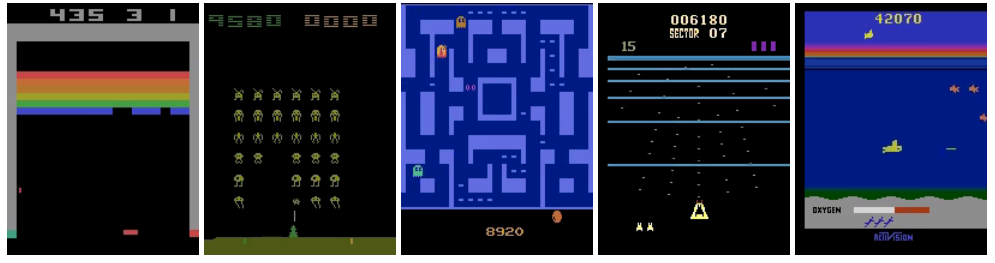
\includegraphics[width=.9\linewidth]{./assets/GYM/gym2}
\caption{Exemple d'environnements GYM (Open AI)}

\bigskip

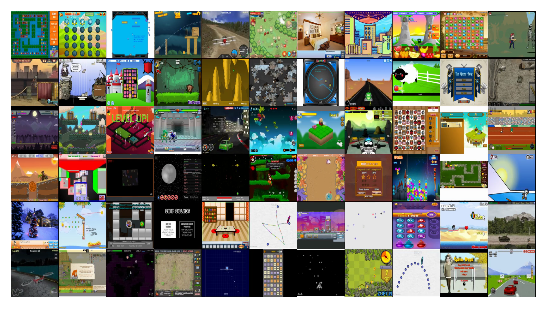
\includegraphics[width=.9\linewidth]{./assets/GYM/gym}
\caption{Exemple d'environnements Universe (Open AI)}

\bigskip

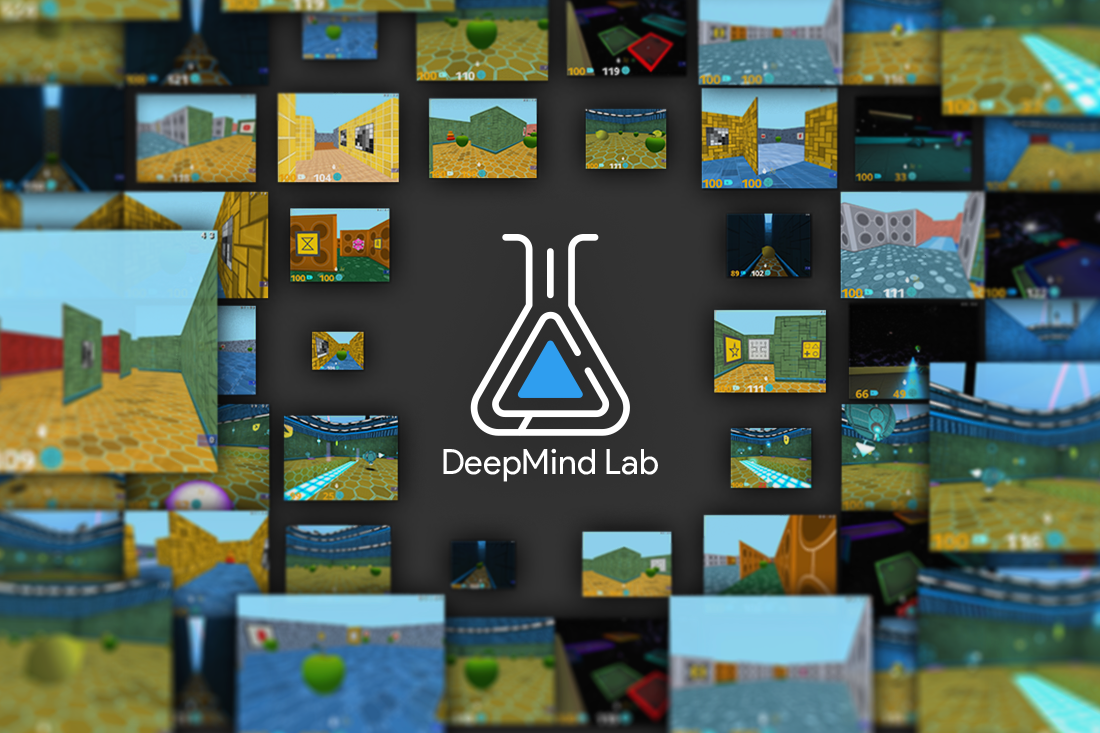
\includegraphics[width=.6\linewidth]{./assets/GYM/deepmindlab}
\caption{Exemple d'environnements DeepmindLab (Deepmind (Google)) }
\medskip
\small
\end{figure}


